
\documentclass[10pt,a4paper,final]{article}
\usepackage[utf8]{inputenc}
\usepackage[english]{babel}
\usepackage{amsmath}
\numberwithin{equation}{section}
\usepackage[font=small,labelfont=bf]{caption}
\newenvironment{Table}
  {\par\bigskip\noindent\minipage{\columnwidth}\centering}
    {\endminipage\par\bigskip}
\usepackage{amsfonts}
\usepackage{amssymb}
\usepackage{makeidx}
\usepackage{graphicx}
\usepackage{lmodern}
\usepackage{hyperref}
\usepackage[left=0.5in,right=0.5in,top=1in,bottom=1in,
						headheight=15pt]{geometry}
\usepackage{blindtext}
\usepackage[bottom]{footmisc}
\usepackage[square, comma, numbers]{natbib}
\usepackage{caption}
\usepackage{subcaption}
\usepackage{fancyvrb}
\usepackage{fancyhdr}
\pagestyle{fancy}
\fancyhead{}
\fancyfoot{}
\fancyhead[L]{Physics 625}
\fancyhead[C]{- - - Ehrenfest Model Writeup - - -}
\fancyhead[R]{Lentner, G.}
\fancyfoot[C]{\large \thepage}
\usepackage{multicol}
\renewcommand{\headrulewidth}{0pt}
\renewcommand{\footrulewidth}{0pt}
\renewcommand{\bibsection}{}


\begin{document}
	
	\thispagestyle{plain}

	\begin{flushleft}
		\LARGE{\textbf{A numerical simulation of the Ehrenfest model of diffusion}}
	\end{flushleft}
	
	\noindent\makebox[\linewidth]{\rule{\textwidth}{0.5pt}}

	\bigskip
		
	\begin{flushright}
	\begin{minipage}[t]{0.85\textwidth}	
		\par{\Large{\textbf{G. Lentner}}\par}
		\bigskip
		\par{\small{\textit{
				LL15 Natural Science Building, University of Louisville,
				Louisville, KY 40292 USA}}\par}
		\par{\small{\textit{
				email: geoffrey.lentner@louisville.edu}}\par}
	\end{minipage}
	\end{flushright}

	\vspace{\baselineskip}

	\begin{flushright}
	\begin{minipage}[t]{0.85\textwidth}
		\textbf{Abstract: } I present here a code for the Ehrenfest model of  \textit{N} 
		particles in two containers. The code is written in C++ and parallelized using
		OpenMP. The parallelization is of iteration and not the simulation. I was able to
		evolve the state of the particles to a Poincare' cycle in modest time. For a 
		system of 28 particles, the code ran 100 iterations in 26.28 minutes using 16 
		threads and measured an average Poincare' cycle of 2.518$\times10^9$ steps. 
		The code is available from it's master online repository: 
		\texttt{\small http://github.com/gLENTNER/EhrenefestModel.git}
	\end{minipage}
	\end{flushright}

	\begin{flushright}
	\begin{minipage}[t]{0.85\textwidth}
		\par{\small{\textbf{Key words: } methods: numerical, statistical}\par}
	\end{minipage}
	\end{flushright}

	\vspace*{2\baselineskip}

	\begin{multicols}{2}[]
		
		\section{Description}

		The code is written in C++ and follows an object-oriented design pattern.
		The primary simulation routine is encapsulated inside a \textit{Model} 
		class. This object takes information from a parsing routine about the
		environment of interest (e.g., number of particles) and follows a system
		from its initial state until either a Poincare' cycle or equilibrium has
		been reached, whichever occurs last. The structure of the code is 
		depicted in Figure~\ref{fig:structure}

		\begin{figure*}[t!]
			\captionsetup{width=0.8\textwidth}
			\centering
			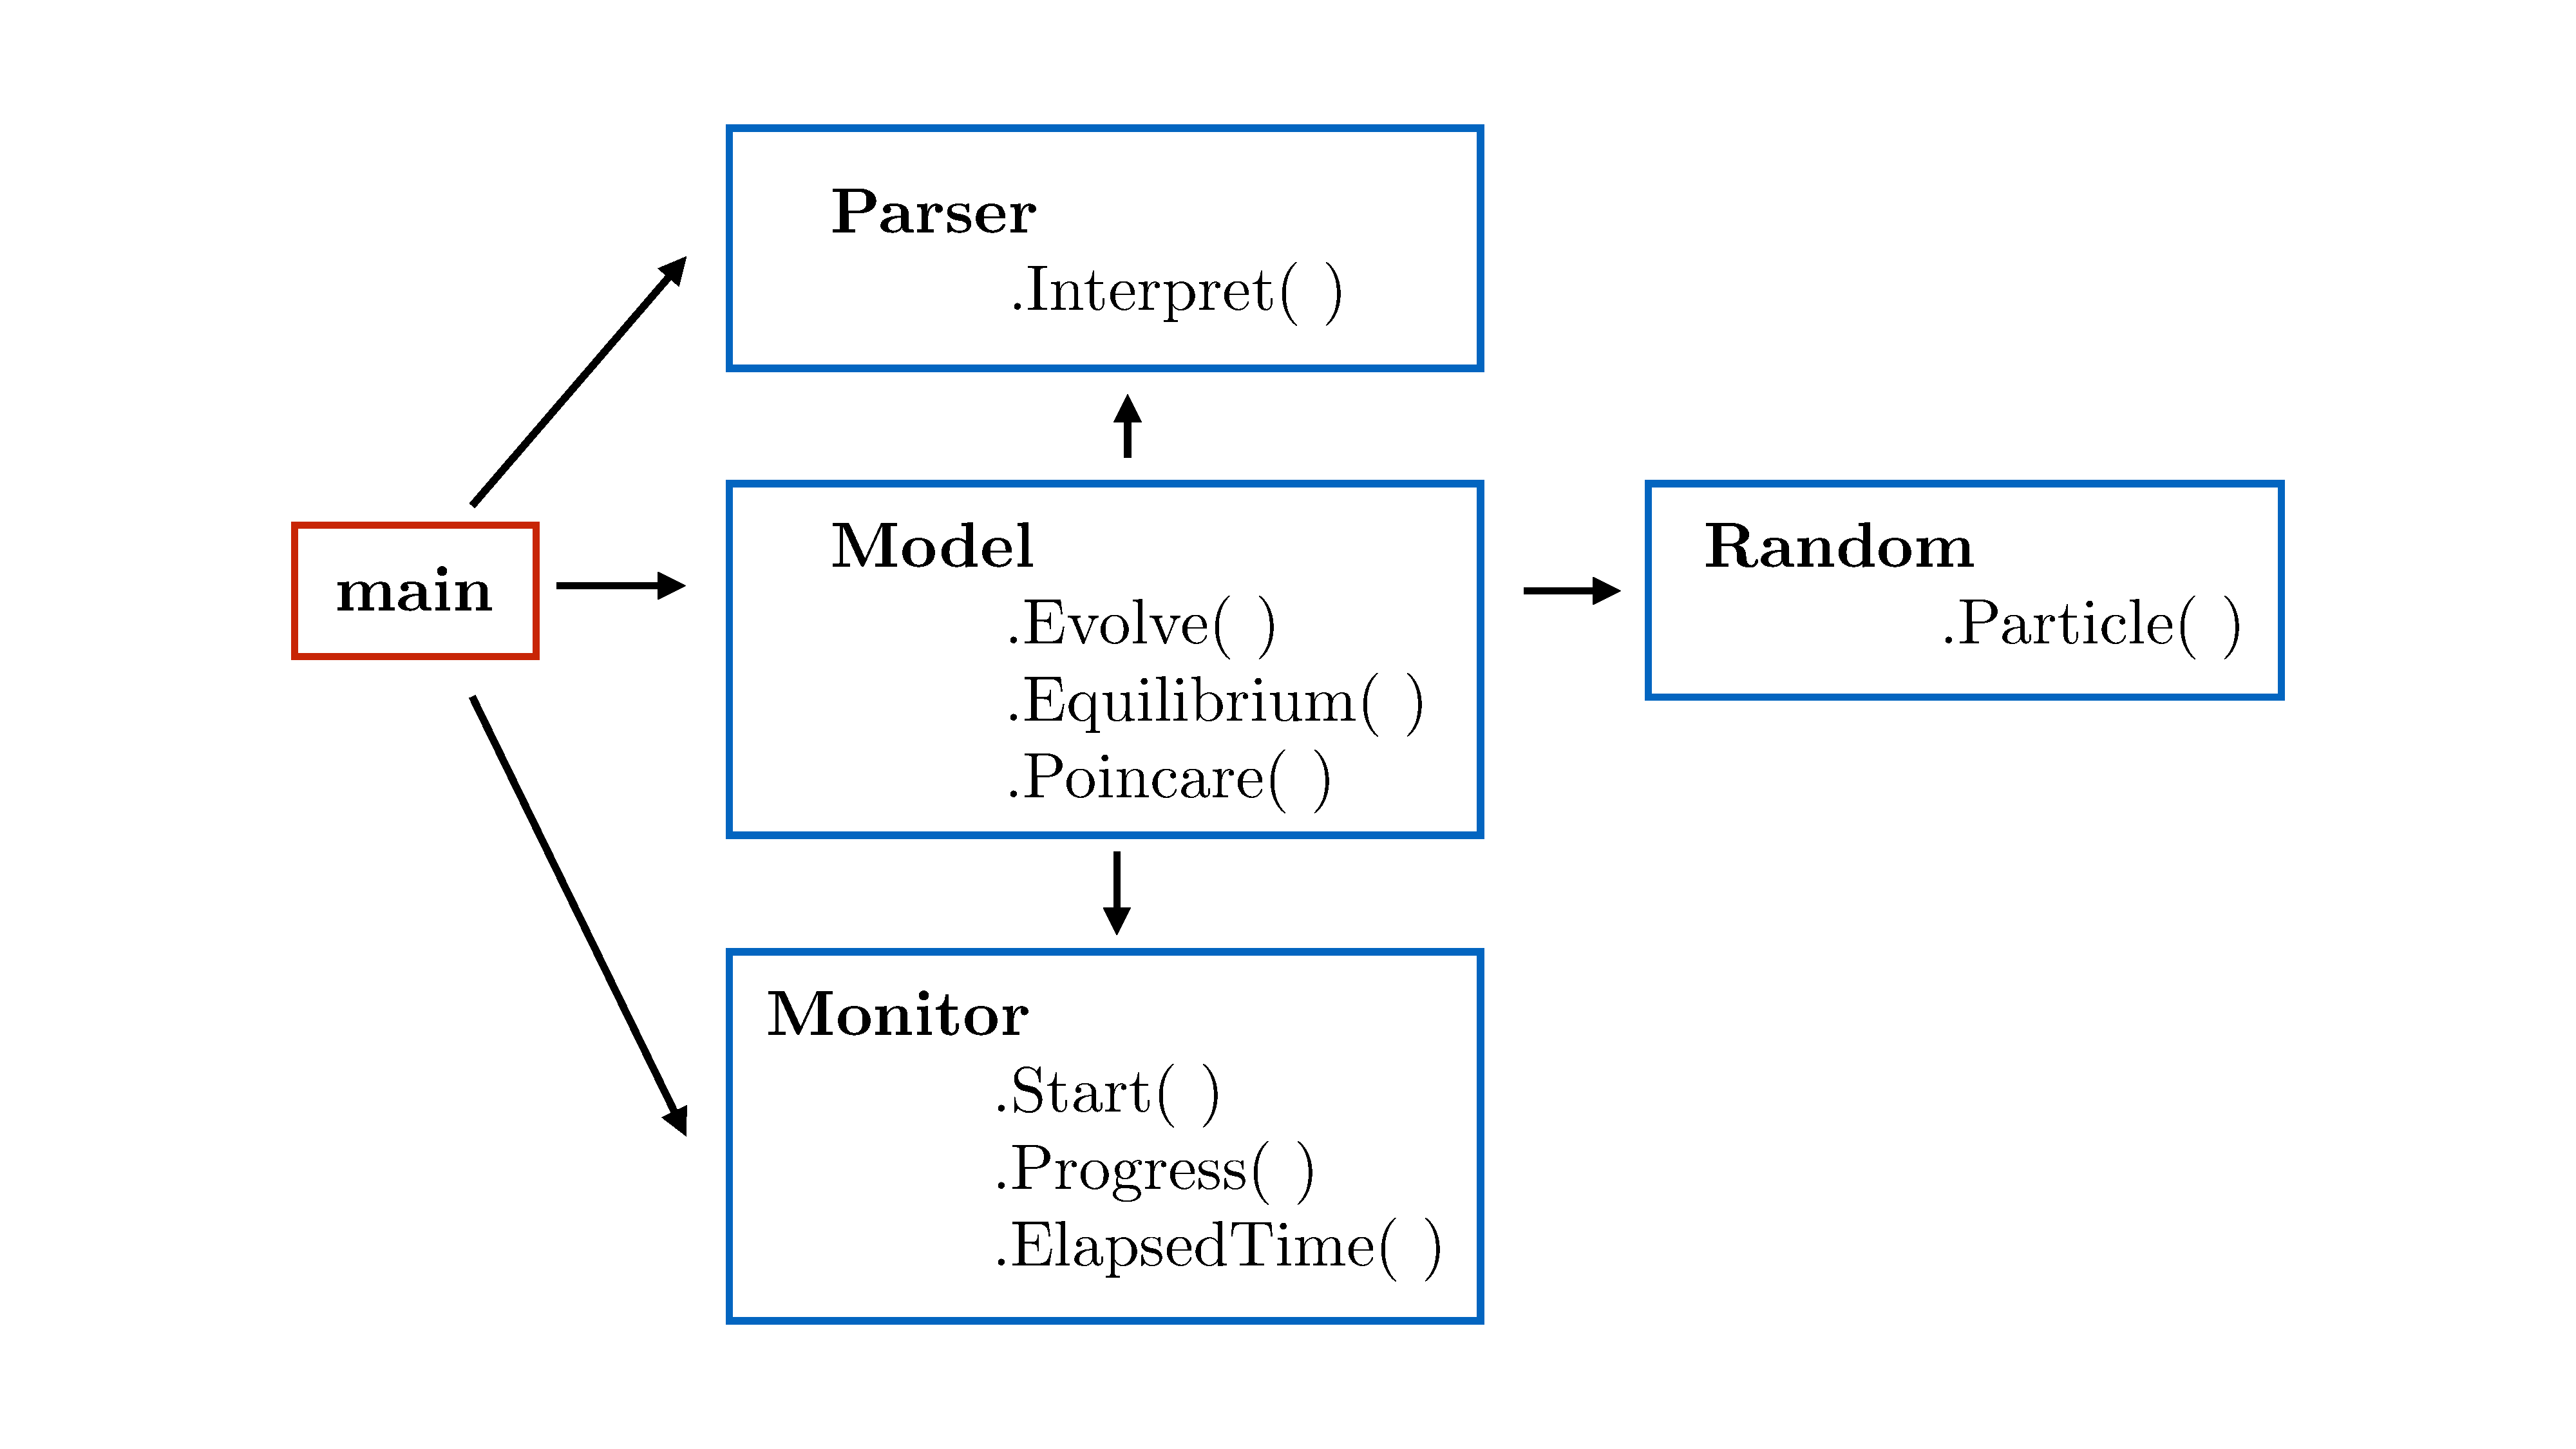
\includegraphics[width=0.8\textwidth]{figures/Structure.pdf}
			\caption{Above is a simplistic structure diagram of the code.
			The elements bordered in blue are part of the}
			\label{fig:structure}
		\end{figure*}


	\end{multicols}

	%	\pagebreak

	\section{Apendix: Source Code}
	\subsection{makefile}
	\VerbatimInput[baselinestretch=1,fontsize=\footnotesize, numbers=left]{../source/makefile}

	\pagebreak
	
	\subsection{main.cc}
	\VerbatimInput[baselinestretch=1,fontsize=\footnotesize, numbers=left]{../source/main.cc}

	\pagebreak
	
	\subsection{GAIAsolution.hh}
	\VerbatimInput[baselinestretch=1,fontsize=\footnotesize, numbers=left]{../source/GAIAsolution.hh}

	\pagebreak

	\subsection{GAIAsolution.cc}
	\VerbatimInput[baselinestretch=1,fontsize=\footnotesize, numbers=left]{../source/GAIAsolution.cc}

	\pagebreak

	\subsection{parser.hh}
	\VerbatimInput[baselinestretch=1,fontsize=\footnotesize, numbers=left]{../source/parser.hh}

	\pagebreak

	\subsection{parser.cc}
	\VerbatimInput[baselinestretch=1,fontsize=\footnotesize, numbers=left]{../source/parser.cc}

	\pagebreak

	\subsection{FileManager.hh}
	\VerbatimInput[baselinestretch=1,fontsize=\footnotesize, numbers=left]{../source/FileManager.hh}

	\pagebreak

	\subsection{FileManager.cc}
	\VerbatimInput[baselinestretch=1,fontsize=\footnotesize, numbers=left]{../source/FileManager.cc}

	\pagebreak

	\subsection{monitor.hh}
	\VerbatimInput[baselinestretch=1,fontsize=\footnotesize, numbers=left]{../source/monitor.hh}

	\pagebreak

	\subsection{monitor.cc}
	\VerbatimInput[baselinestretch=1,fontsize=\footnotesize, numbers=left]{../source/monitor.cc}

	\pagebreak

	\subsection{PopulationManager.hh}
	\VerbatimInput[baselinestretch=1,fontsize=\footnotesize, numbers=left]{../source/PopulationManager.hh}

	\pagebreak

	\subsection{PopulationManager.cc}
	\VerbatimInput[baselinestretch=1,fontsize=\footnotesize, numbers=left]{../source/PopulationManager.cc}
	
	\pagebreak

	\subsection{CDFmanager.hh}
	\VerbatimInput[baselinestretch=1,fontsize=\footnotesize, numbers=left]{../source/CDFmanager.hh}

	\pagebreak

	\subsection{CDFmanager.cc}
	\VerbatimInput[baselinestretch=1,fontsize=\footnotesize, numbers=left]{../source/CDFmanager.cc}

	\pagebreak

	\subsection{PDFbase.hh}
	\VerbatimInput[baselinestretch=1,fontsize=\footnotesize, numbers=left]{../source/PDFbase.hh}

	\pagebreak

	\subsection{MassDensityProfile.hh}
	\VerbatimInput[baselinestretch=1,fontsize=\footnotesize, numbers=left]{../source/MassDensityProfile.hh}

	\pagebreak

	\subsection{MassDensityProfile.cc}
	\VerbatimInput[baselinestretch=1,fontsize=\footnotesize, numbers=left]{../source/MassDensityProfile.cc}

	\pagebreak

	\subsection{MetallicityProfile.hh}
	\VerbatimInput[baselinestretch=1,fontsize=\footnotesize, numbers=left]{../source/MetallicityProfile.hh}

	\pagebreak

	\subsection{MetallicityProfile.cc}
	\VerbatimInput[baselinestretch=1,fontsize=\footnotesize, numbers=left]{../source/MetallicityProfile.cc}

	\pagebreak

	\subsection{HabitabilityProfile.hh}
	\VerbatimInput[baselinestretch=1,fontsize=\footnotesize, numbers=left]{../source/HabitabilityProfile.hh}

	\pagebreak

	\subsection{HabitabilityProfile.cc}
	\VerbatimInput[baselinestretch=1,fontsize=\footnotesize, numbers=left]{../source/HabitabilityProfile.cc}

	\pagebreak

	\subsection{VerticalProfile.hh}
	\VerbatimInput[baselinestretch=1,fontsize=\footnotesize, numbers=left]{../source/VerticalProfile.hh}

	\pagebreak

	\subsection{VerticalProfile.cc}
	\VerbatimInput[baselinestretch=1,fontsize=\footnotesize, numbers=left]{../source/VerticalProfile.cc}

	\pagebreak

	\subsection{TemplateProfile.hh}
	\VerbatimInput[baselinestretch=1,fontsize=\footnotesize, numbers=left]{../source/TemplateProfile.hh}

	\pagebreak

	\subsection{TemplateProfile.cc}
	\VerbatimInput[baselinestretch=1,fontsize=\footnotesize, numbers=left]{../source/TemplateProfile.cc}


	
	
\end{document}	
